\chapter{Optimizing the CNN}\label{make}

\section{(Pre-) processing the dataset}
For the following steps a simulated dataset containing roughly 2.000.000 gamma events and 400.000 hadron events has been used.
Every recorded event holds the count of every arrived photon for all 1440 pixels for 100 consecutively time periods of 5 ns.
To reduce these 144.000 variables all photons have been summed along the time axis for every pixel separately.

Therefore flat greyscale images are being used to train the networks.
The common proceeding of using a separate training, validation and testing dataset will be adapted.
To measure the network's performance the area under the curve score (AUC) is used.
The training of a network is terminated when the AUC-score does not rise anymore (early stopping).


\section{Comparing the network architectures}
At this step every tested network architecture is composed of convolution layers (c)
followed by a pooling layer and fully connected layers (f).
The architecture notation follows this example: A '3c\_2f' architecture translates to a network
starting with three convolution and pooling layers and ending with two fully connected layers.

There are four important hyperparameter for this kind of networks:
The number of images in one batch fed to the network (batch-size)
the size of the patch/kernel in the convolution layer (patch-size)
the number of featuremaps the convolution layer computes (depth)
the number of hidden nodes contained in the fully connected layers (hidden-nodes)
For all parameter a random grid search was performed in the course of the following steps.
To dismiss random fluctuation in the networks performance caused among others by the grid search
fifty networks have been trained for every architecture.

\begin{figure}
    \centering
    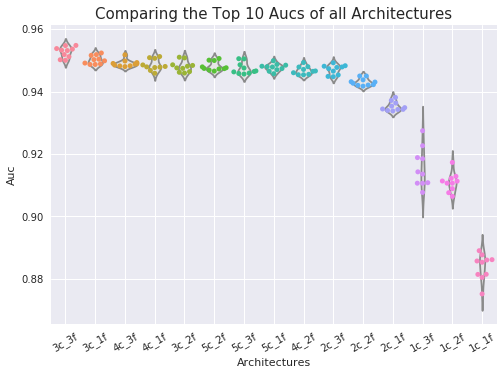
\includegraphics[width=10cm]{Plots/CNN_Architekturen_JMB.png}
    \caption{Comparing the AUCs of the top 10 of every CNN architecture}
    \label{fig:cnn_architectures}
\end{figure}

\begin{figure}
    \centering
    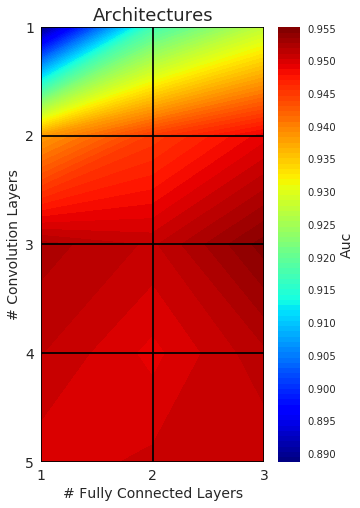
\includegraphics[width=8cm]{Plots/Hyperraum.png}
    \caption{Heatmap of the CNN's performance split by their number of layers}
    \label{fig:heatmap_featurespace}
\end{figure}

Erkenntnis: Tiefer ist besser.

Für weitere Versuche nur noch die besten Netze betrachten



\section{Regularizing the network}
The '3c\_3f' architecture is settled for further investigations to reduce the featurespace to explore.
Integrating a dropout layer extends the options to examine.
There are different possibilities for the position of the layer and
likewise various values for the amount of data to drop out in every layer.

\begin{figure}
    \centering
    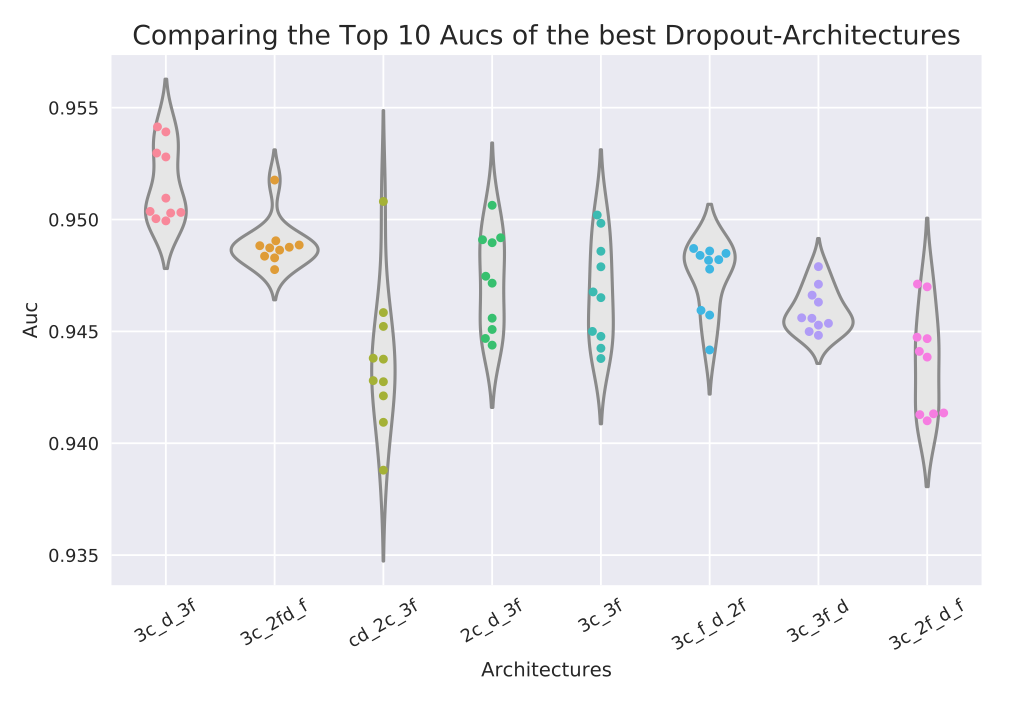
\includegraphics[width=10cm]{Plots/Randomized_Dropout_Model_Comparison.png}
    \caption{Comparing AUCs of different Dropout positions in the CNNs}
    \label{fig:random_dropout}
\end{figure}

Erkenntnis: Convolution muss nicht stark regularisiert werden

Übergang zwischen c-f bietet sich gut an

F-Layer klasse zum dropouten

Pretraining einführen

\begin{figure}
    \centering
    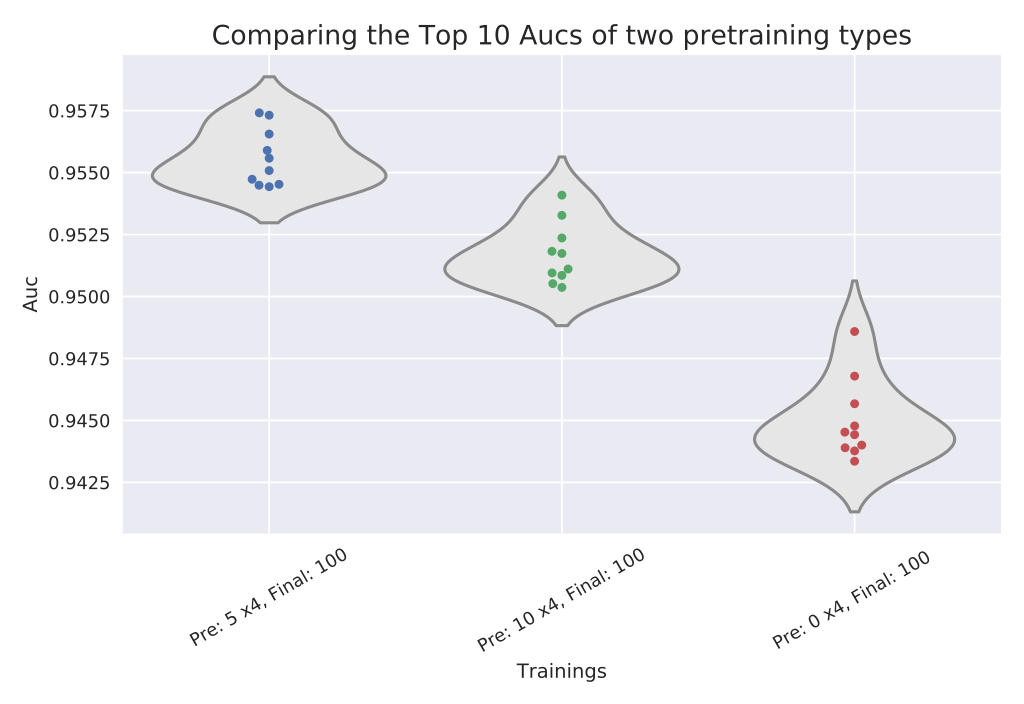
\includegraphics[width=10cm]{Plots/Randomized_Pretraining_Model_Comparison.png}
    \caption{Comparing AUCs of pretrained to normaly trained CNNs}
    \label{fig:random_pretraining}
\end{figure}

Ermöglicht es Netzwerke größerer Tiefe und mit Dropout sicherer zu trainieren

Zeigt robusteres Verhalten

Vergleich mit abgeschnittenem Noise und damit besseren Inputbildern da Event immer in festem Triggerbereich liegt
